\section{Vizualizace}

%\begin{figure}[htbp]
%    \centering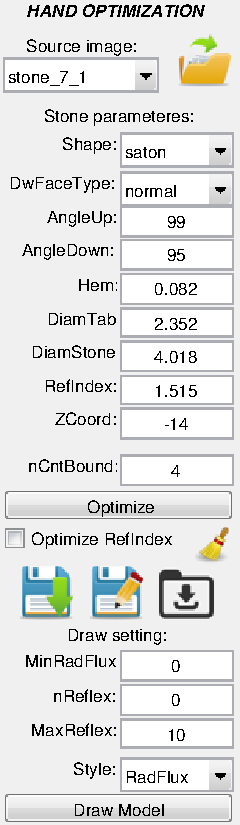
\includegraphics[width=8cm]{controlSaton.pdf}
%     \caption[Filtrace pozadí.]{Filtrace pozadí v HDR snímku znázorněná v jednou řádku obrazu. Od původního signálu je odečteno pozadí, v grafu vyznačeno žlutě.}
%        \label{Detekce}
%\end{figure}
\subsection{Ovládací menu}
\label{sec:ovladaci menu}
GUI program, který umožňuje ruční optimalizace kamene spustíme příkazem \textbf{\textit{handOptimization}}. V prvé řadě je zapotřebí vybrat snímek kamene optimalizovaného kamene. Pokud je snímek ve výchozím adresáři (složka \textit{samples} v kořenovém adresáři programu), lze snímek vybrat z rozbalovacího menu \textit{Source image}. V opačném případě je možnost vybrat snímek ručně přes ikonu 
\includegraphics[width = .35cm]{icons/open-file-icon.png}. Po výběru snímku se zobrazí zdrojový snímek \ref{sec:snimek}.

\begin{wrapfigure}[34]{r}{0.3\textwidth}
\centering
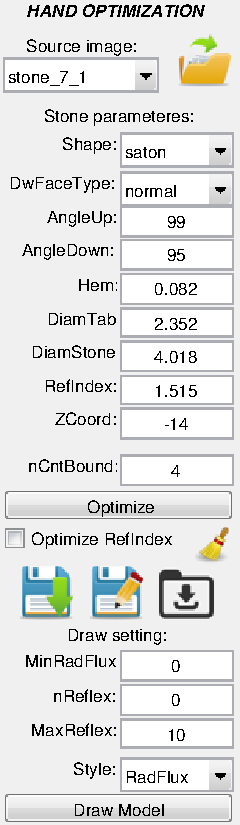
\includegraphics[width=0.3\textwidth]{controlSaton.pdf}
	
\caption[Ruční optimalizace: ovládací menu pro šaton.]{Ovládací menu \textit{handOptimization} pro broušený kámen typu šaton.}
\label{figure:kamera}
\end{wrapfigure}


Dalším postupem je nastavení optimalizovaného kamene. V současné době jsou implementovány broušené kameny tvaru \textbf{viva12}, \textbf{šaton} a \textbf{čtverec}. V první řadě vybereme tvar kamene v kolonce \textit{Shape}. Pod touto kolonkou se zobrazí parametry kamene, které je třeba před optimalizací vyplnit. V případě kamene \textbf{viva12} se jedná o výšku, průměr tabulky a průměr kamene resp. \textit{High}, \textit{DiamTab} a \textit{DiamStone}. Pro kameny \textbf{šaton} a \textbf{čtverec} nastavujeme shodně parametry: typ dolních faset, vrcholový úhel mezi horními a dolními fasetami, velikost lemu (ideálně 0), průměr kamene a průměr tabulky resp. \textit{DwFaceType}, \textit{AngleUp}, \textit{AngleDown}, \textit{Hem}, \textit{DiamTab} a \textit{DiamStone}. Pro všechny typy broušených kamenů nastavujeme navíc index lomu a \textit{z} souřadnici kamene v souřadné soustavě zkalibrované měřicí soustavy resp. \textit{RefIndex} a \textit{ZCoord}. Jednotky rozměrů a souřadnice jsou uváděny v milimetrech, úhly ve stupních. 

Všechny parametry brusu lze měnit i v průběhu optimalizačního procesu. Touto metodou je tedy možné dodatečně určovat neznámé parametry kaneme, úspěch však nelze zaručit. 

Položka \textit{nCntBound} určuje počet odrazů laserového svazku, které se počítají v matematickém modelu. Doporučení je začít s malým číslem a postupně jej navyšovat. %Svazky s každým lomem ztrácí svoji energii, tudíž nejzřetelnější budou svazky s nízkým    

Tlačítkem \textit{Optimize} spustíme optimalizaci náklonu faset kamene, která gradientní metodou nalezne nejlepší model kamen tak, aby směry výstupních svazků modelu odpovídaly směrům přiřazených svazků z experimentálního měření. Ruční přiřazení korespondencí je popsáno v kapitole \ref{sec:snimek}. V případě potřeby se stiskem tlačítka \textit{Z} vrátíme k modelu před optimalizací.  

Výběrem kolonky \textit{Optimize RefIndex} dovolíme optimalizačnímu procesu měnit index lomu kamene. V případě, že je index lomu předem určen doporučuje se index lomu neuvolňovat.

Nalezených korespondence a parametry modelu lze pomocí ikony 
\includegraphics[width = .35cm]{icons/save-icon.png} uložit do stejného adresáře jako vzorový snímek nebo přes ikonu 
\includegraphics[width = .35cm]{icons/save-as-icon.png} vybrat umístění ručně. Uložené výsledky načteme volbou ikony 
\includegraphics[width = .35cm]{icons/load-icon.png}. V průběhu optimalizace můžeme využít užitečné ikony 
\includegraphics[width = .35cm]{icons/clear-icon.png}, která odstaní přiřazené korespondence, pro které v modelu kamene není přítomen odpovídající svazek.  

V ovládacím menu se dále nachází sekce s nastavením hodnot pro vykreslení svazků z modelu kamene do snímku z kamery. Doba vykreslení svazků z modelu kamene závisí na počtu svazků. Pro zmenšení doby vykreslení lze vybrat určitou část svazků, které jsou v oblasti našeho zájmu. Nejen, že se zrychlí doba vykreslení, ale získáme větší přehled mezi modelovanými svazky. 

\begin{figure}[h!]
   \centering
   \begin{minipage}[c]{0.3\textwidth}
     \centering 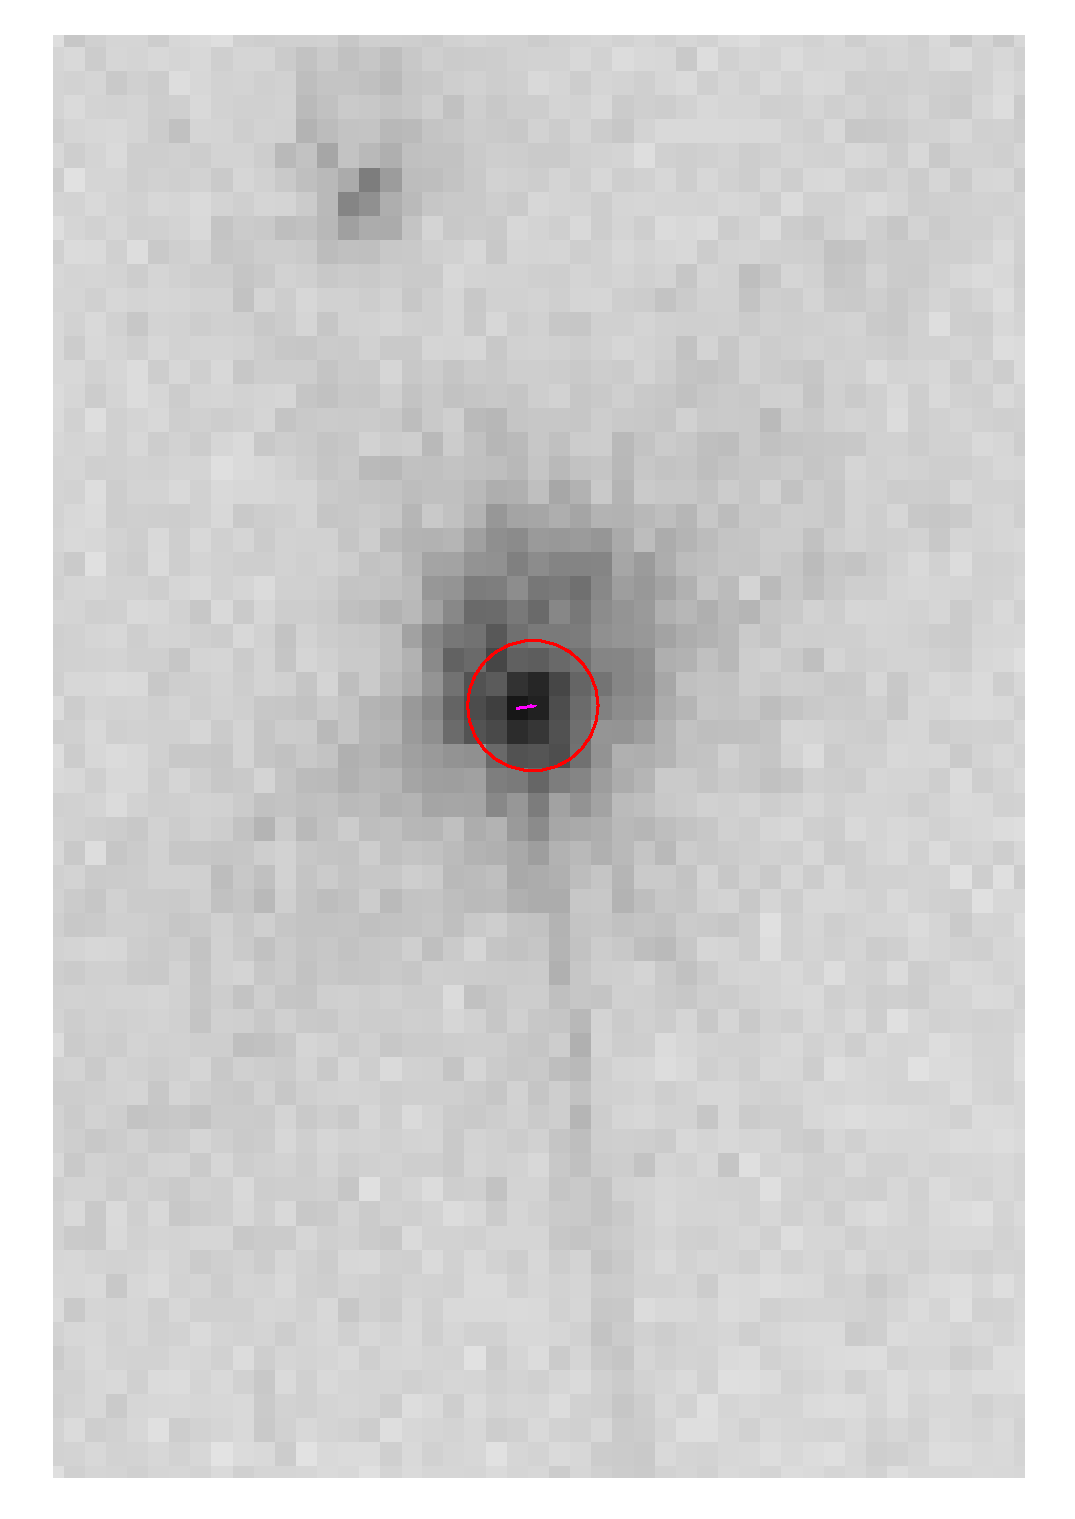
\includegraphics[width=4cm]{radFlux.pdf} 
   \end{minipage}
   \begin{minipage}[c]{0.3\textwidth}
     \centering 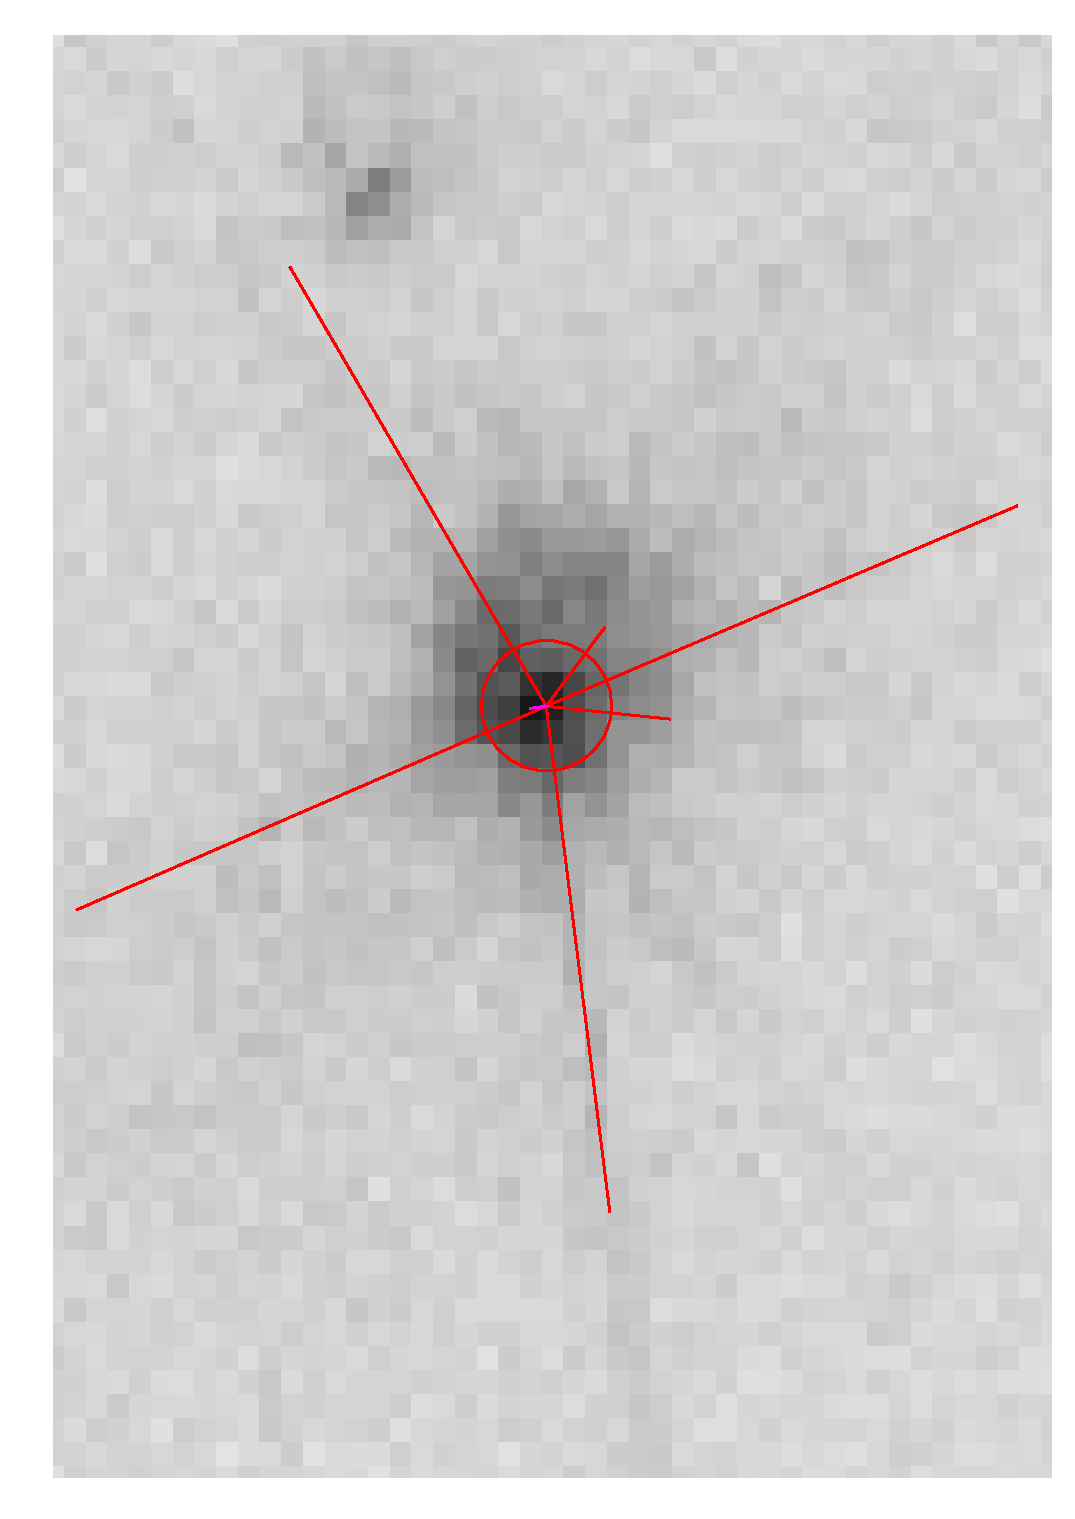
\includegraphics[width=4cm]{tails.pdf} 
   \end{minipage}
   \begin{minipage}[c]{0.3\textwidth}
     \centering 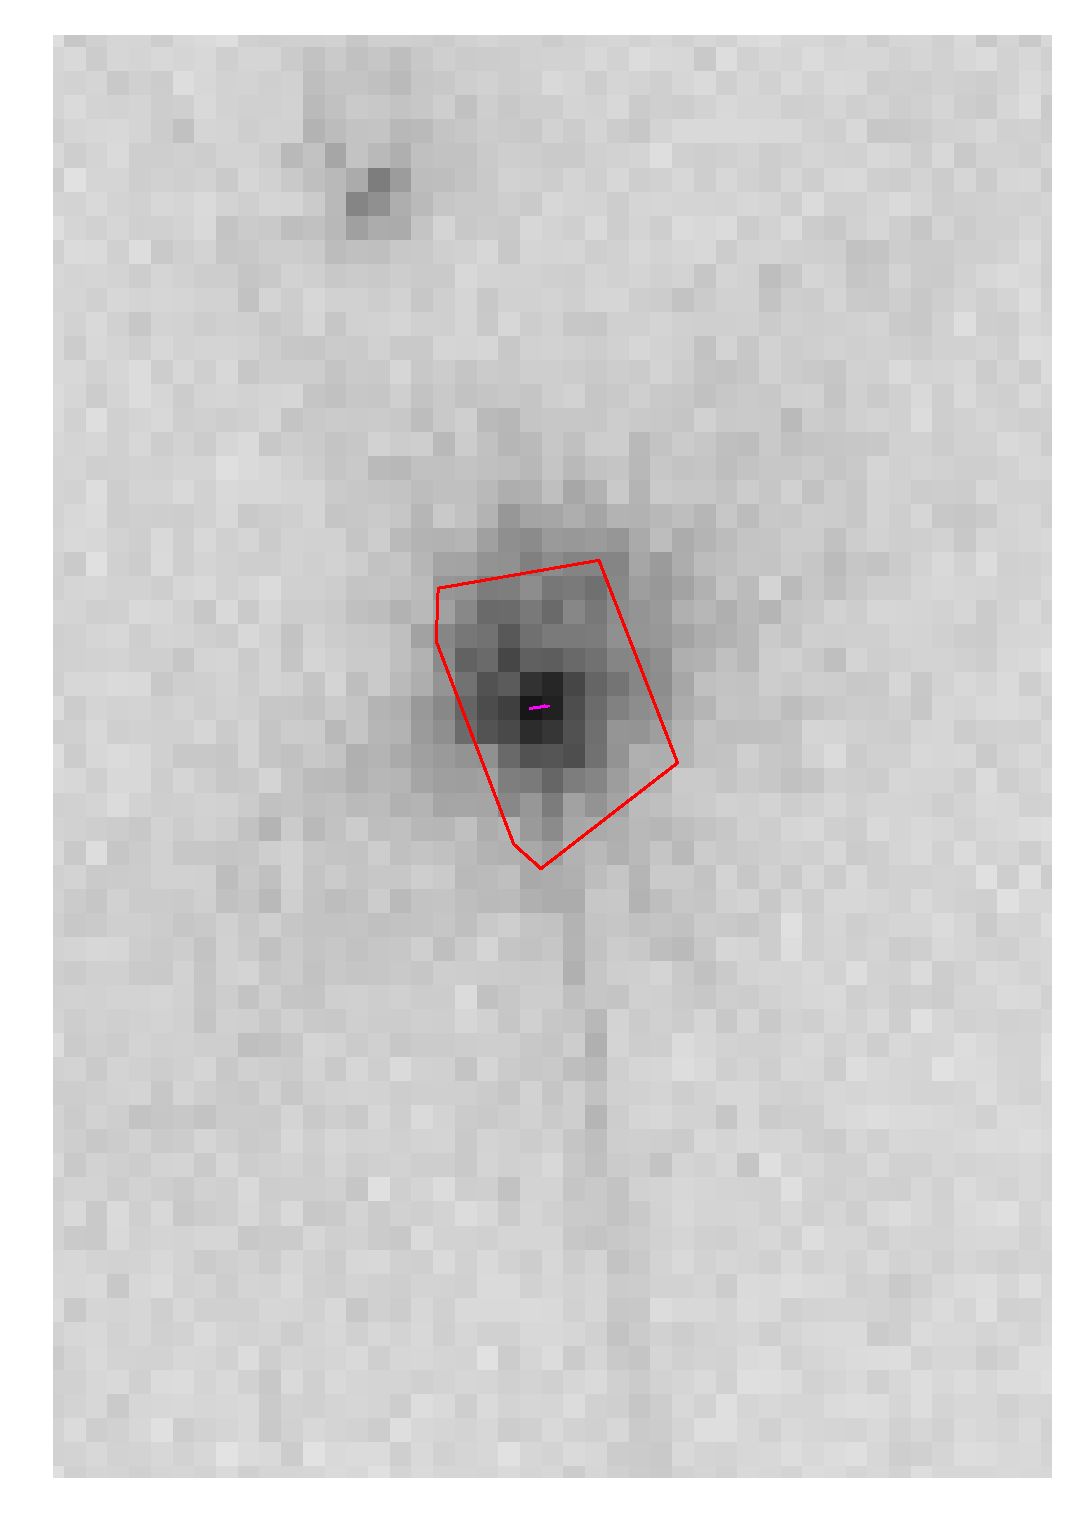
\includegraphics[width=4cm]{polygon.pdf}
   \end{minipage}
   \\
   \caption{Porovnání vykreslovacích stylů. Zleva \textit{RadFlux}, \textit{Tails} a \textit{Polygon}.}
   
\end{figure}

Pomocí kolonky \textit{MinRadFlux} se můžeme omezit pouze na svazky, které mají větší zářivý tok než je určená hranice. Hranici lze nastavovat v intervalu od $0$ do $10000$, což odpovídá odrazu celého laserového svazku od zrcadla. Hodnota \textit{nReflex} určuje výběr svazků s přesným počtem odrazů. Pokud \textit{nReflex} roven $ 0 $ vykreslení není tímto parametrem omezeno. Dále se lze u vykreslení omezit maximálním počtem odrazů svazků, což je omezeno velikostí \textit{MaxReflex}. 

Svazky lze vykreslit třemi různými styly. Výchozí styl \textit{RadFlux} vykresluje velikost svazků podle hodnoty zářivého toku. Styl \textit{Tails} k těmto navíc přidává ocásky, které vzniknou průchodem svazku přes hranu kamene.
Posledním vykreslovacím stylem je styl \textit{polygon}. Zde je na pozici dopadu světelného svazku pomocí polygonu znázorněn tvar svazku po jeho lomu z kamene. Vykreslené svazky kterýmkoliv stylem lze zvětšovat či zmenšovat pomocí klávesnice $+$ resp. $-$.  

Kolonka \textit{Draw Model} slouží k vykreslení aktuálního modelu kamene. 


\subsection{Zdrojový snímek}
\label{sec:snimek}
Po výběru snímku v ovládacím menu \ref{sec:ovladaci menu} se pozadí nového okna zobrazí odpovídající snímek. Přes snímek jsou odpovídajícím stylem (\ref{sec:ovladaci menu}) nakresleny místa dopadů zvolených světelných svazků \ref{sec:ovladaci menu} z aktuálního matematického modelu kamene. 

Okno je nastaveno tak, že reaguje na akce ovládacích prvků na optické myši. Stisknutí levého tlačítka na myši znamená výběr nejbližšího vykresleného svazku. Zobrazí se detekované stopy a vybraný svazek. Opětovným stiskem tlačítka vybereme nejbližší stopu, která spolu se svazkem utvoří korespondující pár. Po spárování se zobrazí opět pouze svazky, kde jsou však barevně odděleny svazky tvořící korespondující pár. Opětovným výběrem svazku, který již byl spárován, odstraníme odpovídající korespondující pár. 

Stiskem pravého tlačítka myši vykreslíme aktuální modle kamene s vyznačenou cestou vybraného svazku.

Změnou polohy kolečka optické myši lze snímek přiblížit či oddálit, což umožňuje snadné zaměření na detaily snímku. 

\begin{figure}[h!]
   \centering
   \begin{minipage}[c]{0.3\textwidth}
     \centering 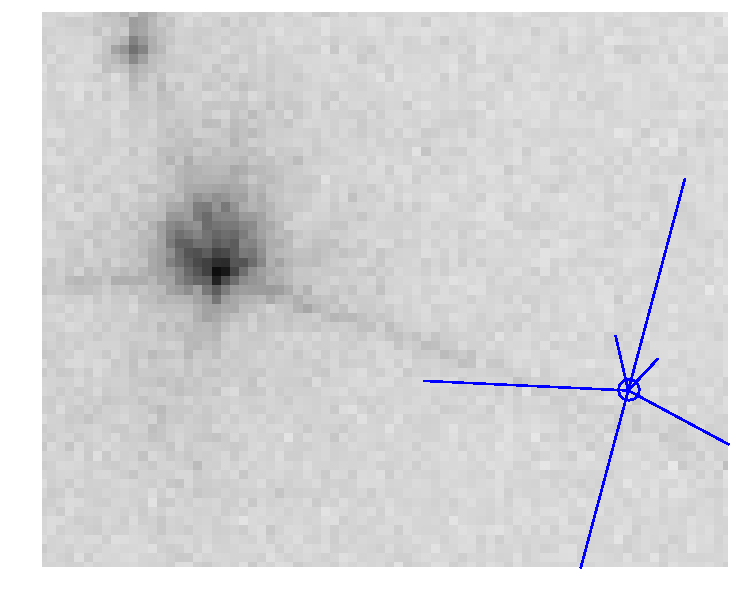
\includegraphics[width=4cm]{empty.pdf} 
   \end{minipage}
   \begin{minipage}[c]{0.3\textwidth}
     \centering 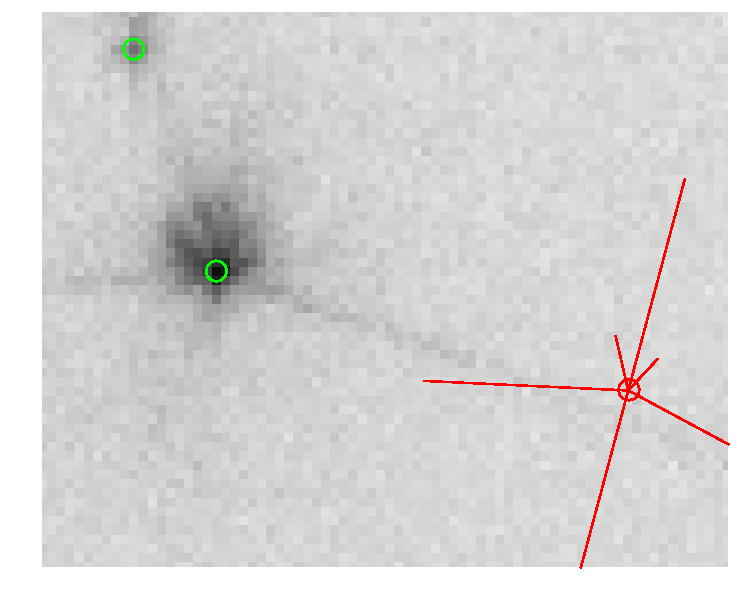
\includegraphics[width=4cm]{choosen.pdf} 
   \end{minipage}
   \begin{minipage}[c]{0.3\textwidth}
     \centering 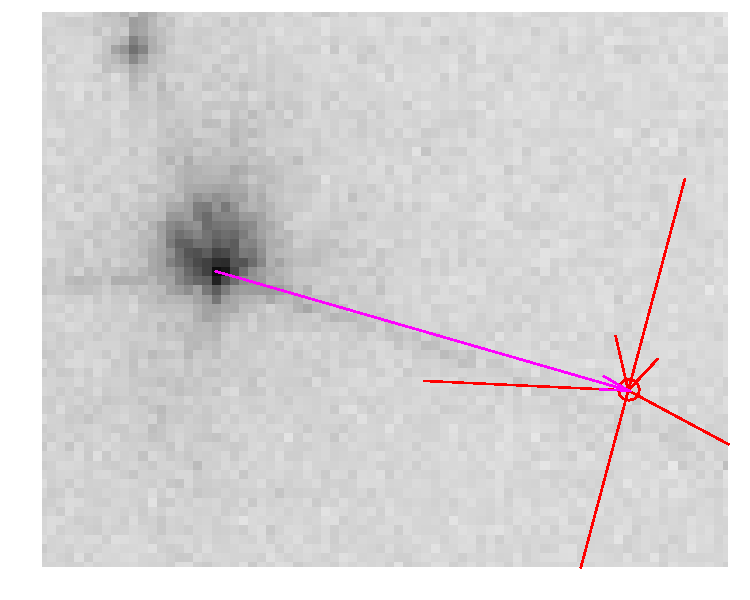
\includegraphics[width=4cm]{pair.pdf}
   \end{minipage}
   \\
   \caption{Ilustrace přiřazení svazku ke stopě. Vlevo volný svazek, uprostřed vybraný svazek a zobrazené stopy a vpravo vytvořený pár svazek/stopa. Vykresleno stylem \textit{Tails}}.
   
\end{figure}

\begin{figure}[h!]
     \centering 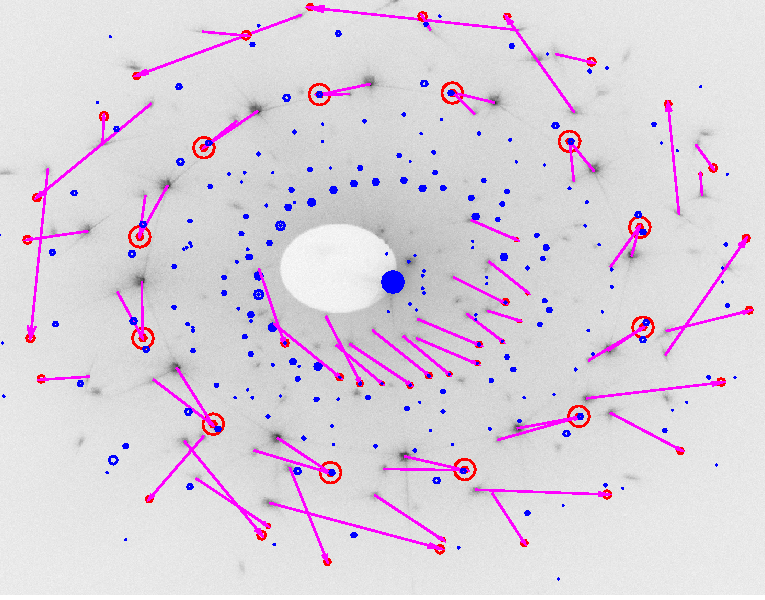
\includegraphics[width=8cm, height = 7.6cm]{initialDistance.pdf} 
   \caption{Vzdálenosti stop od svazků u počátečního modelu. Určit všechny korespondující páry v jednom kroku je prakticky nemožné.}
   \label{fig:initDistance}
   
\end{figure}


\begin{figure}[h!]
     \centering 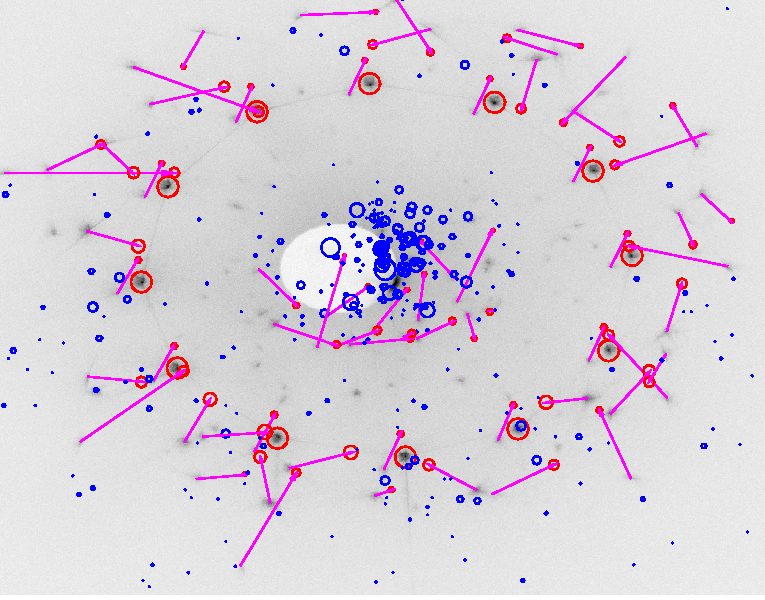
\includegraphics[width=8cm, height = 7.6cm]{distance24_4.pdf} 
   \caption{Vzdálenosti stop po prvním kroku optimalizace. Situace se od obrázku \ref{fig:initDistance} změnila, ovšem stále lze spolehlivě přiřadit pouze některé páry.}
   
\end{figure}



  
%\clearpage